%%%%%%%%%%%%%%%%%%%%% chapter2.tex %%%%%%%%%%%%%%%%%%%%%%%%%%%%%%%%%
%
%  Monotone Circuits Lower bounds 
%
% Use this file as a template for your own input.
%
%%%%%%%%%%%%%%%%%%%%%%%% Springer-Verlag %%%%%%%%%%%%%%%%%%%%%%%%%%
%\motto{Use the template \emph{chapter.tex} to style the various elements of your chapter content.}





\chapter{Monotone Circuit Lower Bounds}
\label{sec:Razborov} % Always give a unique label
% use \chaptermark{}
% to alter or adjust the chapter heading in the running head


% Always give a unique label
% and use \ref{<label>} for cross-references
% and \cite{<label>} for bibliographic references
% use \sectionmark{}
% to alter or adjust the section heading in the running head

We have  seen that proving that SAT is not in \Ppoly, i.e., cannot  be solved by polynomial-size circuits, implies that $\P \neq \NP$.
Due to the notorious difficulty of this and related questions, we are also interested in proving \emph{weaker} lower bounds, namely, lower bounds against \emph{restricted} classes of circuits. Although this does not settle the main lower bound questions, it is still considered an important step towards the bigger questions, at least from the methodological perspective. 
Here, we study such a restricted circuit class and prove a lower bound against it: Boolean circuits without negation gates, which are also called \emph{ monotone circuits}.

\para{Monotone Circuits}

\begin{definition}[Monotone circuit]
A \emph{monotone circuit} is a Boolean circuit that contains fan-in two gates AND and OR, but has \emph{no} NOT gates.
\end{definition}

Note in particular that monotone circuits can compute only monotone functions: a Boolean function is said to be monotone if \emph{increasing the number of ones} in the input cannot flip the value of the function from 1 to 0. More precisely, for $\bar{x}, \bar{y} \in\{0,1\}^n$, write $\bar{x} \geq \bar{y}$ iff $ \forall i \in [n], x_i \geq y_i$, where $[n]$ denotes $\{1,\dots,n\}$. (Here, $x_i\ge y_i$ for Boolean $x_i,y_i$ means simply that $1\ge 0$ and $0\ge 0$, $1\ge 1$, while $0\not\ge 1$.)

\begin{definition}[Monotone function]
A Boolean function $f:\{0,1\}^n \rightarrow\{0,1\}$ is said to be  \emph{monotone} if $\forall \bar{x} \geq \bar{y}, f(\bar{x}) \geq f(y)$.
\end{definition}

\section{The CLIQUE Problem}
Many \NP-complete problems are monotone. One example of an \NP-complete decision problem is  CLIQUE we describe now. 
Given an undirected graph $G=(V, E)$ with $n$ nodes, a \emph{$k$-clique} in $G$ is a set $U\subseteq V$ of size $k$, such that  every pair of nodes $u_1, u_2 \in U$ is connected by an edge (in $E$), and in symbols:
$$
 \forall u_1 \in U~\forall u_2 \in U~ ( u_1 \neq u_2\Rightarrow (u_1, u_2)\in E).
$$


Recall that a computational decision problem is a language over a finite alphabet (usually \bits). Here, our language consists of all the strings that encode (in some natural way) an accepted graph, i.e., a graph with $n$ nodes that contains a $k$-clique.
The natural way to encode a graph in our case is this: a graph  $G=(V, E) $ with $n$ nodes, is encoded by $\binom{n}{2}$ input variables  $x_{ij}$, where the semantic of the encoding is: $x_{i j}=1$ iff $(i, j) \in E$. In other words, if the input variable $x_{ij}=1$,   our input graph contains the edge $(i,j)$, and otherwise it does not. 

We are interested in CLIQUE$(k, n)$ for a \emph{fixed} $k$, considered as the following Boolean function: 
\begin{svgraybox}
The computational problem \textbf{CLIQUE$(k, n)$}: 

\textit{Input}: Undirected graph $G=(V,E)$ with $n$ nodes encoded as a length $n\choose 2$ binary string (each bit represents an  edge  $x_{ij}$, $i<j\in[n]$), and a number $k$ (given in unary, i.e., $1^k$).

\textit{Accept}: if the graph $G$ contains a $k$-clique. 

\textit{Reject}: otherwise.
\end{svgraybox}


 
 
It is known that CLIQUE$(k,n)$ is NP-complete (see standard complexity textbooks; e.g., Papadimitriou 1994).
Note that $\operatorname{CLIQUE}(k, n)$ is a monotone function: if we add 1's to the input, we only \emph{increase} the chance it has a $k$-clique. Since CLIQUE$(n, k)$ is a monotone (Boolean)
function we can compute it by a monotone Boolean circuit. But the question remains whether we can compute CLIQUE$(n, k)$ with small monotone circuit. 

\begin{trailer}{Example of a monotone circuit computing CLIQUE$(n, k)$}
Consider  all $\binom{n}{k} ~~ k$-sub-graphs in $G$, and check if at least one of those is a clique:

\begin{figure}
    \centering
    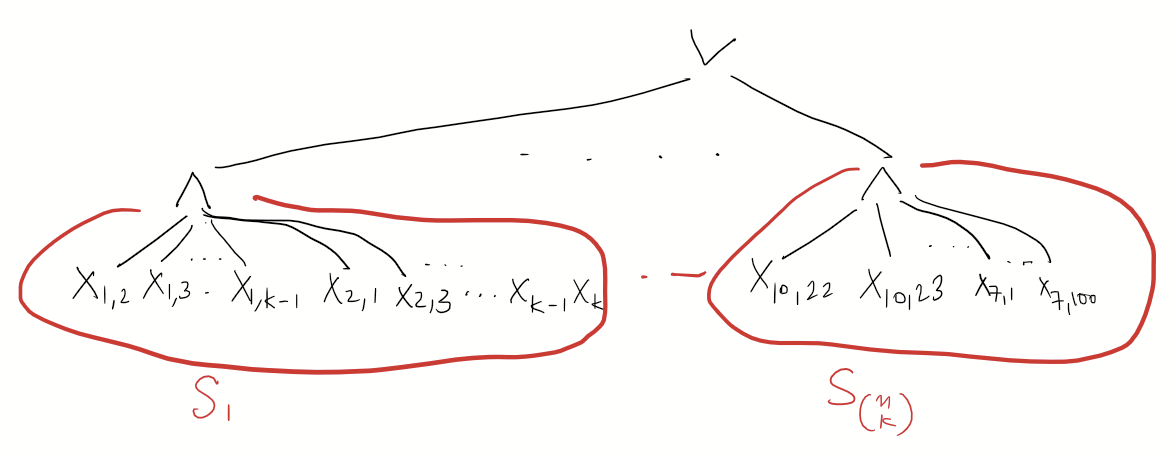
\includegraphics[width=0.75\linewidth]{images/k-clique-simple-circuit.png}
    \label{fig:clique-naive}
    \caption{Naive way to compute CLIQUE}
\end{figure}

$S_1, S_2, \ldots, S_{\binom{n}{k}}$ are the $\binom{n}{k}$ subgraphs in $G$ each of size $k$.
Size of this circuit: $O\left(k^2 \cdot\binom{n}{k}\right)$.
\end{trailer}


\newcommand{\APPX}{\ensuremath{\mathrm{APX}}}



\subsection{Approximators}

A  circuit for computing $\operatorname{CLIQUE}  (n, k),$ consisting of an OR gate $\bigvee$ of many  $S_i$'s, each of size $k$ and where each $S_i$ is an AND of the edge variables in $S_i$, as in the example above, is called an \textit{approximator} for CLIQUE($n, k)$. More formally, we have the following. 

% *Do not* use the \begin{tcolorbox}[float=..] %option, unless you wish it to float around; namely %not appear sequentially as you put in in the %text. 

\begin{tcolorbox}[colframe=white, colback=red!5, boxrule=0mm, sharp corners]
\textbf{Approximators $\APPX\left(X_1, \ldots, X_m\right)$ for CLIQUE}.
Let $V$ be a set of nodes and let $X_1,\dots,X_n\in V$ be a collection of subsets of nodes. The \emph{approximator} $\APPX\left(X_1, \ldots, X_m\right)$ is defined to be 
$\bigvee_{r=1}^m\bigwedge_{i<j \in X_r} x_{ij}$, with $x_{ij}$ the Boolean variables representing that there is an edge between nodes $i$ and $j$.
Note that the $X_i$'s may have different sizes (and specifically their sizes may be different from $k$).
\end{tcolorbox}
 
Note that $\APPX\left(X_1, \ldots, X_m\right)(\alpha)=1$, for $\alpha\in\bits^{n\choose 2}$, precisely when in the graph $G$ over the nodes $V$ described by the assignment $\alpha$, at least one of the $X_i$ subgraphs is a clique. The idea behind the approximator is that it provides a good approximation for the CLIQUE function, in the sense that, depending on the number of sets $m$ and size of each set $X_i$, for many  input graphs it provides the correct answer.   

We shall also use the abbreviated notation $\APPX(\mathcal X)$ for $\APPX(X_1,\dots,X_m)$ when $\mathcal X = \{X_1,\dots,X_m\}$.

% We denote by $\APPX\left(S_1, \ldots, S_{\binom{n}{k}}\right)$ the approximator computing the $\bigvee$ of all subgraphs $S_1, \ldots, S_{n\choose k }$.

\begin{trailer}{Example of simple useful asymptotic computations}
%\begin{note} 
Note that when $k\in(\Omega(\log n),O(n-\log n))$, $\APPX\left(S_1, \ldots, S_{n\choose k}\right)$, where $S_1,\dots,S_{n\choose k}$ are all possible subsets of size $k$ from the set of $n$ nodes $V$, is of \emph{super-polynomial size}, because $ n\choose k$ is super polynomial for $k$ in this range. For the sake of getting used to asymptotic estimates such as these, it is helpful to go over the computations in more detail, as follows.

We shall estimate the asymptotic behaviour of $\binom{n}{\log n} $, showing it is superpolynomial, namely, $\binom{n}{\log n} =
n^{\Omega(\log n)}$. First, we observe that

$$\binom{n}{k} \ge\left(\frac{n}{k}\right)^k. $$
To prove this lower bound we do the following.
Write $\binom{n}{k}=\frac{n!}{k!(n-k)!}=
\frac{\prod_{j=0}^{k-1}(n-j)}{k!}=\prod_{j=0}^{k-1} \frac{n-j}{k-j}$. Notice that each factor $\frac{n-j}{k-j}$ in this product is at least $\frac{n}{k}$, and there are $k$ factors, giving the lower bound $\left(\frac{n}{k}\right)^k$. 

Now, to lower bound $\binom{n}{\log n} $ we have:

\[  
\begin{aligned}
 \binom{n}{\log n} \geq\left(\frac{n}{\log n}\right)^{\log n}
& =
\left(
    \frac{2^{\log n}}
        {2^{\log (\log n)}}\right)^{\log n} \\
& =2^{(\log n-\log \log n) \cdot \log n} \\
& =2^{\log^2n-\log n \cdot \log \log n} \\
& =2^{\log ^2 n-o(\log ^2n)} \\
& = 2^{c \log ^2 n} \text {, ~~~for some constant $c$, say, $c=1/2$} \\
& =\left(2^{\log n}\right)^{c \cdot \log n}=
n^{c \log n},
\end{aligned}
\]
which means that $\binom{n}{\log n}= n^{\Omega(\log n)}$.



% ------------------ Using Stirling

% Stirling's approximation for factorials helps simplify the expressions: 
% \begin{tcolorbox}[colframe=white, colback=gray!5, boxrule=0mm, sharp corners]
% \textbf{Stirling's Approximation}:
% $n!\sim \sqrt{2 \pi n}\left(\frac{n}{e}\right)^n$, where $e$ is the natural logarithm.
% \end{tcolorbox}
% 
% By definition, we have $\binom{n}{\log n} =\frac{n!}{\log n!(n-\log n)!}$. Hence, using Stirling's approximation to substitute the factorials we get:
% \[
%  \binom{n}{\log(n)} \sim \frac{\sqrt{2 \pi n} \left(\frac{n}{e}\right)^n}{\sqrt{2 \pi \log(n)} \left(\frac{\log(n)}{e}\right)^{\log(n)} \sqrt{2 \pi (n - \log(n))} \left(\frac{n - \log(n)}{e}\right)^{n - \log(n)}}.
% \]
%  
% Simplifying, we combine the square root terms:
%    \[
%    \frac{\sqrt{2 \pi n}}{\sqrt{2 \pi \log(n)} \sqrt{2 \pi (n - \log(n))}} \sim \frac{1}{\sqrt{2 \pi \log(n)}}.
%    \]
% Simplify the exponentials:    the \(\left(\frac{n}{e}\right)^n\) term dominates the numerator, and dividing by \(\left(\frac{\log(n)}{e}\right)^{\log(n)}\) and \(\left(\frac{n - \log(n)}{e}\right)^{n - \log(n)}\) leads to:
% 
%    \[
%    \left(\frac{n}{n - \log(n)}\right)^{n - \log(n)} \cdot \left(\frac{n}{\log(n)}\right)^{\log(n)}.
%    \]
% 
% For large \(n\), \(n - \log(n) \sim n\), namely, $n-\log (n) =\Omega(n)$, so:
%  $
%    \left(\frac{n}{n - \log(n)}\right)^{n - \log(n)} \sim 1.
%  $
% Hence, the dominant term becomes $\left(\frac{n}{\log(n)}\right)^{\log(n)}.$
% Thus 
% \[
% \binom{n}{\log(n)} \sim \frac{1}{\sqrt{2 \pi \log(n)}} 
% \cdot \left(\frac{n}{\log(n)}\right)^{\log(n)}
% \ge  \left(\frac{n}{\log(n)}\right)^{c\log(n)}, 
% \]
% ======
%=========================================== 
% % for some constant $c$, and all sufficiently large $n$'s.
% % This is the same as writing
% %\[
% %\binom{n}{\log(n)} 
% %=  \left(\frac{n}{\log(n)}\right)^{\Omega(\log(n))}. 
% %\]
% %
% Using the fact that $2^{\log(\log n)}=\log n$,  we get:
% \begin{align*}
% \binom{n}{\log n} & \ge 2^{c\cd\log n\cd(\log n-\log(\log n))}\\
% &   = 
% 2^{c\cd\log n\cd\log n-c\cd\log n \cd\log(\log n))}\\
% &   = 
% 2^{c\cd\log^2 n-o(\log ^2n)}\\
% &   =
% 2^{\Omega(\log^2(n))} = n^{\Omega(\log n)}.
% \end{align*}

\end{trailer}
% 
% To asymptotically estimate \(\binom{n}{\log(n)}\), we can use the binomial coefficient formula and apply approximations for large \(n\). The binomial coefficient is defined as:
% 
% \[
% \binom{n}{k} = \frac{n!}{k!(n-k)!}.
% \]
% 
% Here, \(k = \log(n)\), where we assume the logarithm is base 2 unless specified otherwise. For large \(n\), this becomes:
% 
% \[
% \binom{n}{\log(n)} = \frac{n!}{(\log(n))!(n - \log(n))!}.
% \]
% 
% ### Using Stirling's Approximation
% Stirling's approximation for factorials (\(n! \sim \sqrt{2 \pi n} \left(\frac{n}{e}\right)^n\)) helps simplify the expressions. Applying this:
% 
% 1. For \(n!\):
%    \[
%    n! \sim \sqrt{2 \pi n} \left(\frac{n}{e}\right)^n.
%    \]
% 
% 2. For \((\log(n))!\):
%    \[
%    (\log(n))! \sim \sqrt{2 \pi \log(n)} \left(\frac{\log(n)}{e}\right)^{\log(n)}.
%    \]
% 
% 3. For \((n - \log(n))!\):
%    Since \(n - \log(n) \sim n\) for large \(n\), we approximate:
%    \[
%    (n - \log(n))! \sim \sqrt{2 \pi (n - \log(n))} \left(\frac{n - \log(n)}{e}\right)^{n - \log(n)}.
%    \]
% 
% ### Substituting
% Now substitute these approximations into the binomial coefficient:
% 
% \[
% \binom{n}{\log(n)} \sim \frac{\sqrt{2 \pi n} \left(\frac{n}{e}\right)^n}{\sqrt{2 \pi \log(n)} \left(\frac{\log(n)}{e}\right)^{\log(n)} \sqrt{2 \pi (n - \log(n))} \left(\frac{n - \log(n)}{e}\right)^{n - \log(n)}}.
% \]
% 
% ### Simplifying
% 1. Combine the square root terms:
%    \[
%    \frac{\sqrt{2 \pi n}}{\sqrt{2 \pi \log(n)} \sqrt{2 \pi (n - \log(n))}} \sim \frac{1}{\sqrt{2 \pi \log(n)}}.
%    \]
% 
% 2. Simplify the exponentials:
%    The \(\left(\frac{n}{e}\right)^n\) term dominates the numerator, and dividing by \(\left(\frac{\log(n)}{e}\right)^{\log(n)}\) and \(\left(\frac{n - \log(n)}{e}\right)^{n - \log(n)}\) leads to:
% 
%    \[
%    \left(\frac{n}{n - \log(n)}\right)^{n - \log(n)} \cdot \left(\frac{n}{\log(n)}\right)^{\log(n)}.
%    \]
% 
%    For large \(n\), \(n - \log(n) \sim n\), so:
%    \[
%    \left(\frac{n}{n - \log(n)}\right)^{n - \log(n)} \sim 1.
%    \]
% 
%    The dominant term becomes:
%    \[
%    \left(\frac{n}{\log(n)}\right)^{\log(n)}.
%    \]
% 
% ### Final Asymptotic Estimate
% Thus, the leading-order asymptotic behavior of \(\binom{n}{\log(n)}\) is:
% 
% \[
% \binom{n}{\log(n)} \sim \frac{1}{\sqrt{2 \pi \log(n)}} \cdot \left(\frac{n}{\log(n)}\right)^{\log(n)}.
% \]
% 
% This grows extremely rapidly as \(n\) increases.

% ===========================
% end Stirling computation 
% 

\section{Clique is hard for monotone circuits }
The following theorem shows the naive (brute-force) way of computing the CLIQUE function with a monotone circuit shown in Figure \ref{fig:clique-naive}    cannot be improved much.

\begin{figure}
    \centering
    
\includegraphics[width=0.3\linewidth]{images/RAZBOROV_Alexander.jpeg}
    \caption{Alexander Razborov. Creator: Kozloff, Robert | Credit: Photo by Robert Kozloff.
Copyright: The University of Chicago}
    \label{fig:enter-label}
\end{figure}


\begin{tcolorbox}[colframe=white, colback=blue!5, boxrule=0mm, sharp corners]
\begin{theorem}[Razborov~\cite{Razb85}; cf.~\cite{AB87}]\label{thm:razborov} Let $k=\sqrt[4]{n}$. Then, every monotone circuit computing {\rm CLIQUE}$(n, k)$ has size $2^{\Omega(\sqrt[8]{n})}$.
\end{theorem}
\end{tcolorbox}
That is, there exists a constant $c$ such that  for large enough $n \in \mathbb{N}$, if $C_n$ computes CLIQUE$(n,k)$ then $\left|C_n\right| \geq 2^{c \cdot \sqrt[8]{n}}$.


The rest of this chapter aims to prove this theorem. \textit{Our exposition is taken mostly from Papadimitriou's textbook} \cite{Pap94}.


%Recall: a approximator is a big OR of cliques, each computed as a big AND.




\section{Proof of monotone circuit lower bounds \Cref{thm:razborov} using the Approximation Method}


\paragraph{Approximation Method Overview}

We first provide an overview of the approach we take to prove \Cref{thm:razborov} which is called \emph{the approximation method}. 
We shall describe a way of approximating any \textbf{monotone} circuit for $\operatorname{CLIQUE}({n}, {k})$ by a approximator, namely a big OR of cliques, as follows.
 

\begin{tcolorbox}[colframe=white, colback=blue!5, boxrule=0mm, sharp corners]
\textbf{Approximation Method}:
The upshot of the method is the following: \emph{by  way of contradiction,} consider a purported small monotone circuit computing  $\operatorname{CLIQUE}({n}, {k})$, and show by induction, gradually progressing from the input nodes towards the output node, that the function computed at every gate can be well approximated by a small approximator. Then, if the number of nodes in the circuit is small the output gate is also well approximated by a small approximator. Now, use an auxiliary argument to show that there is no small approximator approximating well  $\operatorname{CLIQUE}({n}, {k})$.
\end{tcolorbox}
% =======
% The upshot is the following: \emph{by way of contradiction,} consider a purported small monotone circuit computing  $\operatorname{CLIQUE}({n}, {k})$, and show by induction, gradually progressing from the input nodes towards the output node, that the function computed at every gate can be approximated by a small approximator. Then, the output gate is also approximated by a small approximator. Now, use an auxiliary argument to show that there is no small approximator approximating $\operatorname{CLIQUE}({n}, {k})$.
% >>>>>>> f39d2195a6351cafba5750ac78532621d361fb0c

More precisely, we have:  
\begin{enumerate}
 
\item  Given a monotone circuit $C$, we shall construct a approximator 
$\APPX(X_1, \ldots, X_m)$ for some $m$ and $|{X}_{i}| \leq l$ (for some $l$, and for $i=1, \ldots, m$ ), that approximates $\operatorname{CLIQUE}({n}, {k})$ with \textbf{precision} that is dependent on the number of gates in $C$.
% =======
% \item  Given a monotone circuit $C$, we shall construct a approximator ${\APPX}({X_1, \ldots, {X_m})}$ for some $m$ and $\left|{X}_{{i}}\right| \leq l$ (for some $l$, and for ${i}=1, \ldots, {m}$ ), that approximates $\operatorname{CLIQUE}({n}, {k})$ with \textbf{precision} that is dependent on the number of gates in $C$.
% >>>>>>> f39d2195a6351cafba5750ac78532621d361fb0c

\item That is, if the number of gates in $C$ is small the precision is  good, namely the approximator ${\APPX}(X_1, \ldots, X_m)$ for $\operatorname{CLIQUE}({n}, {k})$ we end up with makes \textit{few} mistakes on the $\operatorname{CLIQUE}({n}, {k})$ function (a mistake happens when the circuit  answers  "NO" on an input that has a $k$-clique, or "YES" on an input that has no $k$-clique).\label{it:approximation-b}

The \textbf{approximation} (i.e., construction of an approximator for CLIQUE(${n},{k})$ given the circuit $C$) will proceed in steps, one step for each gate of the monotone circuit:

\begin{enumerate}
    
\item If $C$ is a monotone circuit computing $\operatorname{CLIQUE}({n}, {k})$ we can \textit{approximate} any gate OR or AND in $C$ with an approximator.

\item Each such approximation step introduces rather few errors (false positives and false negatives).
\end{enumerate}



\item We show that every approximator ${\APPX}({X}_1, \ldots, {X_m})$ ($|{X}_i| \leq l$ for some $l$, for all $i=1, \ldots, m$ ), ought to make \textit{exponentially many errors} on the function $\operatorname{CLIQUE}(n, k)$. From \ref{it:approximation-b} above we conclude that there exists no circuit $C$ with a small number of gates. 
\end{enumerate}





\begin{trailer}{Parameters \& notation}

Recall we want to compute CLIQUE$(n, k)$
with $n$ the number of nodes in the graph and $k$ the size of a clique within the graph. 
Throughout the proof, from now on we set:
$$
k=\sqrt[4]{n}.
$$


$$
\begin{aligned}
& l=\sqrt[8]{n} \\
& p \approx \sqrt[8]{n} \\
& M=(p-1)^l \cdot l! & \approx(\sqrt[8]{n}-1)^{\sqrt[8]{n}} \cdot(\sqrt[8]{n})! \\
& & \leq(\sqrt[4]{n})^{\sqrt[8]{n}}.
\end{aligned}
$$


Each (hypothetical) approximator we use in the approximation is:

$$
\APPX\left(X_1, \ldots, X_m\right)
$$

for $m \leq M$ and $\left|X_i\right| \leq l, \forall i \in[m]$.
\end{trailer}

\newcommand{\cliquenk}{\ensuremath{\operatorname{CLIQUE}(n,k)}}

%___________________________________________________________________
\subsection{The Input Set: Extreme Graphs, False Positive and  Negatives}
%___________________________________________________________________

Here we consider the input graphs we are going to analyse. 
The input set to the \cliquenk\ function are \emph{all possible} binary strings of length $n\choose 2$, namely, all possible (encodings) of undirected graphs with $n$ nodes. This set is easily divided into two groups:

\begin{description}
\item[Accept-instances:] 
$G=(V, E)$ is a graph on $n$ modes that contains a $k$-clique.
\item[Reject-instances:]
$G=(V, E)$ is a graph on $n$ nodes that does not contain a $k$-clique.
\end{description}


 



A crucial point is that \emph{we are going to restrict attention only to a special \textbf{subset} of all possible input graphs}. We call these special input graphs \emph{extreme graphs}. 

\para{Extreme Graphs}
We  restrict attention to only a subsets of accept and reject instances. This is sufficient for the proof (and simplifies it). 
Because extreme graphs are part of the input set, a correct circuit clearly must answer correctly on this subset. So, if we show that there must be mistakes made by small circuits on this subset of input graphs, it is immediate that there is no small monotone circuit that correctly computes \cliquenk.



Thus, our focus is on ``extreme'' cases of inputs:

\begin{description}
\item[\textbf{Positive-inputs}:] 
 $G=(V,E)$ has $n$ nodes and a $k$-clique (i.e., a set of $k$ nodes with all edges between them); while \emph{no} other edge exist in $G$ except for the $k$-clique.

There are $\binom{x}{k}$ positive-inputs, each one is clearly an accept input to \cliquenk.
For simplicity, we shall call these positive inputs \emph{$k$-\textbf{cliques}} (although these are special extreme cases of $k$-cliques, since we assume that all edges outside the clique are absent.) 

\begin{figure}[H]
    \centering
    \includegraphics[width=.5\linewidth]{images/clique1.png}
    \caption{Example of a \emph{positive input}: a graph whose only edges are part of a (single) $k$-clique.}
    \label{fig:enter-label}
\end{figure}


\item[\textbf{Negative-inputs}:] 

$G=\left(V,E\right)$ has $n$ nodes and a $(k-1)$-colouring. I.e., $k-1$ independent sets (each with its own distinct colour), namely sets of nodes, such that in each set there are no edges between nodes. Moreover,  \emph{all} edges between nodes in  different independent sets are present!
For simplicity, we shall call these negative inputs \emph{$(k-1)$-\textbf{colouring}} (although these are special extreme cases of $k-1$-colourable graphs, since we assume that all edges between independent sets are present). 


\begin{figure}[H]
    \centering
    \includegraphics[width=.6\linewidth]{images/clique2.png}
    \caption{Example of a \emph{negative input} (i.e., $k-1$-colouring): a graph whose all and only edges are between distinct $(k-1)$-independent sets.}
    \label{fig:enter-label}
\end{figure}

\end{description}

\begin{note}\

\begin{enumerate}
\item There are $(k-1)^n$ negative -inputs. (We count twice two identical graphs with colours interchanged.

\item 
 A $(k-1)$-colouring is a negative-input for \cliquenk\ because a $k$-clique cannot be coloured by $k-1$ colours.
\item
 Assuming each independent set has at least one node (namely,
there exist  $k-1$ nodes with different colours) then even a \emph{single} \emph{edge} added to a $(k-1)$-colouring will make the graph contain a $k$-clique!
\end{enumerate}
\end{note}

\para{False Positive and False Negative Inputs}

Let $V$ be a set of $n$ nodes, and  $\APPX(\mathcal X)$ be an   approximator, with  $\mathcal X$ a collection $X_1\dots,X_m\subseteq V$ of subsets of nodes. We say that  a graph $G(V,E)$ (with $n$ nodes) is a \textbf{false positive} if $\APPX(\mathcal X)(G)=1$ while $G$ is  a $(k-1)$-colouring (and hence, not a $k$-clique). Similarly, a graph $G$ with $n$ nodes $V$ is said to be a \textbf{false negative} if $\APPX(\mathcal X)(G)=0$ while $G$ \emph{is} a $k$-clique.


%___________________________________________________________________
%\subsection{Approximating $\lor,\land$ Gates with approximators %}
%___________________________________________________________________





%\begin{tcolorbox}[colframe=white, colback=red!4, boxrule=0mm, sharp %corners]
%\begin{lemma}[Approximating ]
%\label{lem:}
%
%\end{lemma}
%\end{tcolorbox}


%___________________________________________________________________
\subsection{Concluding the Lower Bound using Structural Induction    }
%___________________________________________________________________



% Recall that our goal is:
% 
% \begin{tcolorbox}[colframe=white, colback=blue!1, boxrule=0mm, sharp corners]
% \textbf{Goal}: Show that every monotone circuit computing $\operatorname{CLIQUE}(n,k)$ has size at least $2^{c \sqrt[8]{n}}$ for some constant $c$ (for sufficiently large $n$).
% \end{tcolorbox}



What does it mean that an approximator $\APPX(\mathcal X)$ \emph{approximates} the monotone circuit C? It means that ``on most'' extreme input graphs $G$, $C(G) = \APPX(\mathcal X)(G)$, namely the approximator agrees with the actual circuit on most $G$'s. 

The approximation of the  monotone circuit $C$ that computes $\operatorname{CLIQUE}(n, k)$ is constructed  by\emph{ induction on the size of $C$,} i.e., number of $\lor, \wedge$ gates in $C$.


\begin{tcolorbox}[colframe=white, colback=gray!11, boxrule=0mm, sharp corners]
\begin{note} Such an induction is usually called \emph{\textbf{induction on the structure of the circuit} $C$} (or \emph{structural induction}), since we are going to induce on subcircuits of $C$, assuming the induction hypothesis holds for them. Using the structure of the circuit, we shall conclude that the induction hypothesis  holds for the gate that connects those two subcircuits. The base case is showing that the induction statement holds for circuits of size 1 (i.e., singled variable circuits). The induction step is showing that the induction statement holds for $A\lor B$ assuming the induction statement holds for both $A$ and $B$. And similarly for the case of $A\land B$.     
\end{note}
\end{tcolorbox}

 

Now, assume that $C$ is a monotone circuit we wish to build an approximation for. We are going to build the approximator for the output gate $C$ gradually, from the input gates of $C$  through the internal gates, up to the output gate, so that the approximator of the output gate will be the approximator of the circuit $C$. The skeleton of this construction is done as follows, following a standard structural induction scheme:


\newcommand{\gapx}{\ensuremath{{\rm approx}}}

\begin{trailer}
{Approximation of the output gate of $C$ via structural induction}

Recall that $\APPX({\mathcal X})$ stands for an approximator with the parameters described above $ l=\sqrt[8]{n} , p \approx \sqrt[8]{n}, M=(p-1)^l \cdot l!$.
For every gate $g$ in $C$ we are going to define $\gapx(g)$ to be $\APPX(\cX)$ for some sequence $\cX$ of sets of nodes, i.e., an OR of cliques $\cX$. The main challenge would be to define precisely which sets $\cX$ are used for each gate approximator, which will be done in the sequel.


\begin{description}
\item[\textbf{Base Approximation Step}:] 
Input nodes $x_{ij}$. Define the approximator of $x_{ij}$, denoted  to be precisely $x_{ij}$, that is $\gapx(x_{ij}):=x_{ij}$.
Note that $x_{ij}$ is indeed an OR of (a single) AND, namely $x_{ij}=\APPX(\{x_{ij}\})$, and so this definition is legit.

\item[\textbf{Induction  Approximator Step}:]\

\case 1 OR gate $g_1\lor g_2$. By induction hypothesis we already built the approximators of $g_1,g_2$, $\gapx(g_1),\gapx(g_2)$, respectively. Using these, we construct an approximation of $g_1\lor g_2$ denoted $\gapx(g_1\lor g_2)$  (we shall show how to define this approximator as $\APPX(\cX)$ in the  sequel).

\case 2 AND gate $g_1\land g_2$. 
By induction hypothesis we already built the approximators 
of $g_1,g_2$, $\gapx(g_1),\gapx(g_2)$, respectively. 
We construct an approximation of $g_1\land g_2$ denoted 
$\gapx(g_1\land g_2)$ from these (again, we shall do this in the sequel).
\end{description} 
\end{trailer}


 %We call the two cases of the induction step above \emph{the approximator steps}. Namely, we have an approximator step for an OR gate and an AND gate, respectively. 


\begin{definition}[Introducing new false positives and false negatives]
Let $g_1\circ g_2$ be an $\lor$ or $\land$ gate with two incoming subcircuits $g_1$ and $g_2$, respectively (i.e., $\circ\in\{\lor,\land\}$). And let $x_{ij}$ be in input node in the circuit (with no incoming edges).
\begin{itemize}
\item 
For \emph{every} graph $G$, whether a positive or a  negative instance, 
$\gapx(x_{ij})(G)=(x_{ij})(G)$, hence we say that \emph{neither a false positive nor a false negative was introduced}.  
 
\item 
Let the graph $G$ be a \emph{negative} input, i.e., a $(k-1)$-colouring. If $(\gapx(g_1)\circ \gapx(g_2))(G)=0$, namely, $\gapx(g_1)\circ \gapx(g_2)$ correctly identified $G$ as a negative input, 
while $\gapx(g_1\circ g_2)(G)=1$, we say the approximator 
step \emph{\textbf{introduced $G$ as a new false positive}}. 

\item Let the graph $G$ be a \emph{positive} input, i.e., a $k$-clique. If $(\gapx(g_1) \circ \gapx(g_2))(G)=1$, namely, $\gapx(g_1)\circ \gapx(g_2)$ correctly identified $G$ as a positive input, while 
$\gapx(g_1\circ g_2)(G)=0$, we say the approximator 
step \textbf{\emph{introduced $G$ as a new false negative}}.
\end{itemize}
\end{definition}

Notice the  subtlety in this definition: introducing new errors here means that we do not care for errors introduced before, namely, those errors incurred  when we constructed each of the (separate) approximators for $g_1$ and $g_2$. We only count \emph{new errors introduced over the function computed by $\gapx(g_1)\circ \gapx(g_2)$}.


%\begin{note}
%Make sure to notice that an approximation of a gate $g_1\land g_2$ is an approximation of appx(g) AND appx(h), where we prove that the approximation of g AND h is good because it introduces on top of the errors incurred already by appx g   as well as  appx h, only few *new* errors. 
%\end{note}





To prove the lower bound theorem, all we need to know are \emph{some properties} of the approximator steps. In other words, given these properties it would not be important how precisely we defined the approximators for gates (that is, how precisely we picked the $\cX$ in each approximator $\APPX(\cX)$).
In particular, the following two lemmas, proved in the next section, are sufficient to conclude the proof. 
\begin{lemma}\label{lem:new-false-positives}
Each approximation step introduces at most $M^2 \cdot \frac{(k-1)^n}{2^p}$ false positives.
\end{lemma}

\begin{lemma}\label{lem:new-false-negatives}
Each approximation step introduces at most $M^2 \cdot\binom{n-l-1}{k-l-1}$ false negatives.
\end{lemma}


Given these two lemmas, we can now relatively easily conclude the lower bound. The idea is that, if we assume by way of contradiction that we are given a small monotone circuit computing \cliquenk, then we can approximate the output gate of this circuit with an approximator that does not make too many errors: the circuit is small and each original gate when approximated contributes only a few new errors. But it is not hard to show that a good approximator for the \cliquenk\ function does not exist. We formalise this argument in what follows.





\bigskip









\begin{proof}[of \Cref{thm:razborov}, given  \Cref{lem:new-false-positives} and \Cref{lem:new-false-negatives}]
\

We use the following claim. 

\begin{claim}\label{cla:internal-in-monotone-lower-bound}
 Every approximator  \APPX$\left(X_1, \ldots, X_m\right)$ with 
  $\left|X_i\right| \leq l$ and $m \leq M$ is either identically 0, that is, an OR of \emph{zero} ANDs, which is the formula $0$ (and thus is wrong on all positive instances, namely all positive instances are false negatives in this case), or outputs 1 on at least half of the (extreme) negative instances (namely, at least half of the negative instances are false positives).

\end{claim}
\begin{proof}
If $\operatorname{\APPX}\left(X_1 \ldots X_m\right)$ is not identically 0 (namely, not the OR of \emph{zero} ANDs, i.e., not the formula $0$), then it accepts at least those graphs $G$ that have cliques on at least one of the sets $X_i$, for some $i\in[m]$. The size of $X_i$ is at most $ l<k$, thus many graphs $G$ that are not $k$-cliques still have $l$-cliques, which may cause the approximator to evaluate to 1 when there is a $|X_i|$-clique on the nodes in $X_i$.


In Figure \ref{fig:R(xi)}  we see an example. The subset $X_i$ is circled in green and contain four nodes. To fool the approximator to accept a $k-1$-colouring, the $k-1$-colouring should contain a clique on the four nodes in $X_i$, which means that each node in $X_i$ is assigned a different colour and hence sent to a distinct independent set. The figure shows an example where this happens: the five independent sets are circled in red, and no two nodes in $X_i$ live in the same independent set. Hence, there is a clique on all nodes in $X_i$.
\begin{figure}[H] 
    \centering
    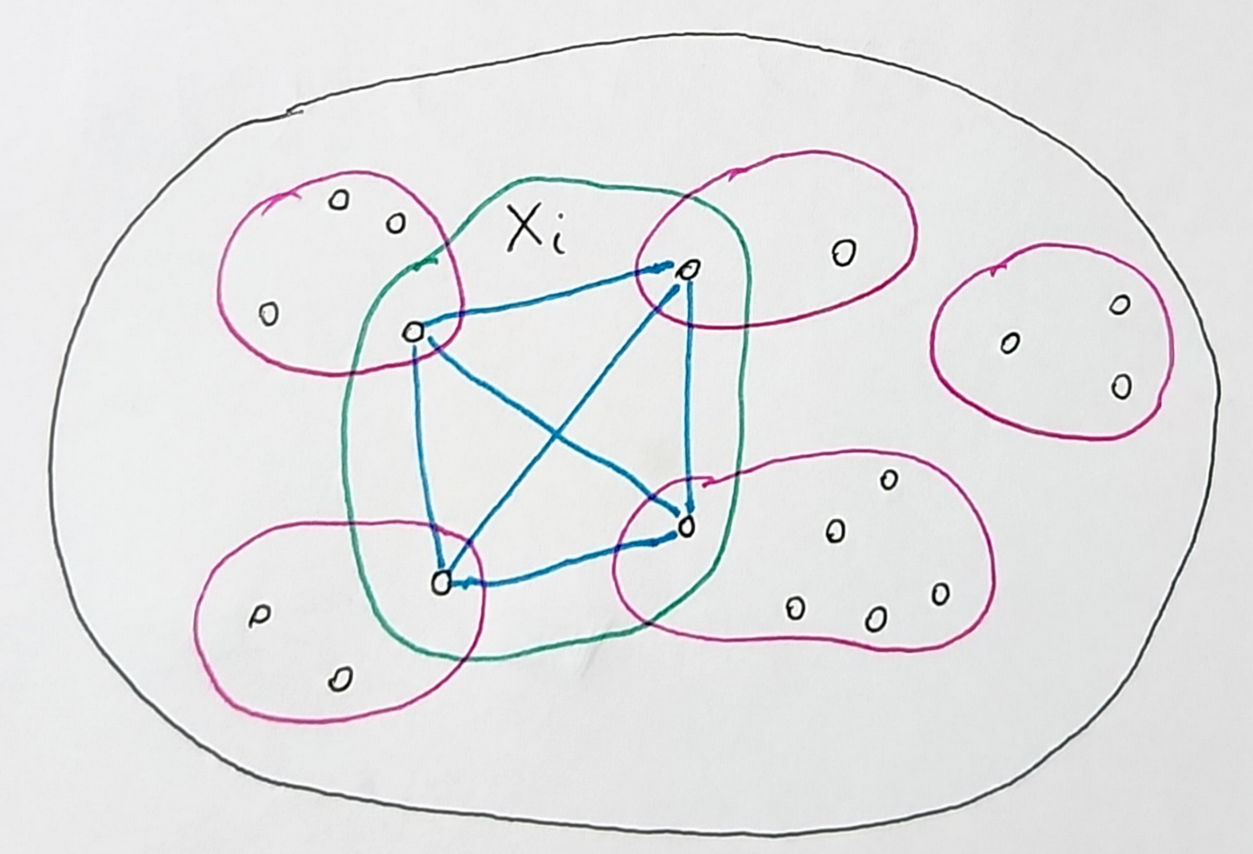
\includegraphics[scale=0.35]{images/R(Xi)-lemma-cliques.png}
        \caption{Example of a $k-1$-colouring that fools an approximator that checks for a clique on  the set $X_i$. The red sets are the independent sets, the green set is $X_i$ and the blue edges are the clique formed on $X_i$ that fools the approximator $\operatorname{\APPX}\left(X_1, \ldots, X_m\right)$.}
    \label{fig:R(xi)}
\end{figure}

Let us  estimate  how many such extreme graphs exist. 
Namely, we wish to show that there are many negative instances, i.e., $k-1$-colourings, that will nevertheless satisfy  
$\operatorname{\APPX}\left(X_1 \ldots X_m\right)$.
It is simple to estimate this using \emph{probability}. Consider a graph $G=(V, E)$ and  assign randomly (and independently) from among $k-1$ colours to the nodes of $G$. Let $v_1 \neq v_2 \in V$ be two nodes, then we  have
$$
\operatorname{Pr}\left[\text { colour of } v_1=\text { colour of } v_2\right]=\frac{1}{k-1},
$$
because regardless of the colour $v_1$ got, there is only one colour out of $k-1$ options for $v_2$ that will match the colour of $v_1$.

Denote by $R\left(X_i\right)$ the event that in the random colouring of $G$, there exists a pair of nodes with the same colour in $X_i$.
Then, 
$$
\operatorname{Pr}\left[R\left(X_i\right)\right] \leq \frac{\binom{|X_i |}{2}}{k-1} \leq \frac{\binom{l}{2}}{k-1} \leq \frac{1}{2}.
$$
The first inequality from the left holds using the union bound and the fact that there are $\binom{\mid X_i |}{2}$ pairs
of nodes in $X_i$. See below for a recap of the union bound and basic notions from discrete probability we shall use throughout this book.
The rightmost inequality holds because 
$ \frac{\binom{\sqrt[8]{n}}{2}}{\sqrt[4]{n}-1}
= \frac{\frac{\sqrt[8]{n} \cdot(\sqrt[8]{n}-1)}{2}}{\sqrt[4]{n}-1} \le \frac{\sqrt[4]{n}}{2\sqrt[4]{n}}=\frac{1}{2}.
$



This means that out of all negative instances to CLIQUE $(n, k)$ (namely, all $(k-1)$-colourings with $n$ nodes), at least half of them are going to colour $X_i$ with \emph{different} colours. Hence, for these negative instances, there will be edges between all nodes in $X_i$, and thus for each of these negative instances $G$ we have $\APPX\left(X_1, \ldots, X_m\right)(G)=1$.
\end{proof}




\begin{tcolorbox}[colframe=white, colback=green!4, boxrule=0mm, sharp corners]
\textbf{Union Bound}: if in a random experiment
there are $m$ possible ``bad'' events, each with probability at most $\alpha$, then the probability that at least one of the ``bad'' events occurred is at most $m\alpha$.

\small
\medskip 
---

We recall some  basic notions from  \textbf{discrete (finite) probability}, and explain more formally the union bound in what follows.

In discrete probability we consider a \emph{ Sample Space}
$\Omega$ as a finite set of  all possible outcomes of a random experiment. The experiment is random in the sense that its outcomes are not deterministic rather hold  probabilities. 
Each element $a$ in $\Omega$ is a possible outcome of the  random experiment, and is sometime called an \emph{atomic outcome}, and  holds a precise probability denoted $\Pr\left[a \right]$, such that:
\begin{enumerate}
\item $0\le \Pr\left[a\right]\le 1$, for all $a\in\Omega$.

\item $\Sigma_{a\in\Omega}\Pr[a]=1$.
\end{enumerate} 

An \emph{event} is a set $E\subseteq\Omega$ of atomic outcomes. The probability of an event $E\subseteq\Omega$ is naturally defined as $\Sigma_{a\in E}\Pr[a]$. 


\bigskip 
The \emph{union bound} provides an upper bound on the probability of the union of multiple events. Formally, if \( E_1, E_2, \dots, E_n \) are events in a probability space, the union bound states:

\[
P\left(\bigcup_{i=1}^n E_i\right) \leq \sum_{i=1}^n P(E_i)
\]

Intuitively, the union bound tells us that the probability of at least one of the events \( E_1, E_2, \dots, E_n \) occurring is at most the sum of the probabilities of each individual event. This bound is useful because it is often \emph{much easier} to calculate or estimate the probabilities of \emph{individual} events than to calculate the exact probability of their union.

 If some events are not disjoint, their combined probability is generally less than the sum of their probabilities, so the union bound is not tight in this case. The union bound is tight (exact) if and only if the events are disjoint. Otherwise, it overestimates the probability due to double-counting overlaps among the events.




\end{tcolorbox}

We are now ready to conclude the proof of \Cref{thm:razborov} (given the two lemmas \ref{lem:new-false-positives} and \ref{lem:new-false-negatives}).
Recall that $l=\sqrt[8]{n}$ and
let $p=\sqrt[8]{n} \cdot \log n$. 
Thus, 
\begin{equation}
\label{eq:651:16}
\begin{aligned}
M  = 
(p-1)^l \cdot l!
& \leq (\sqrt[8]{n} \cdot \log n)^{\sqrt[8]{n}} \cdot \sqrt[8]{n}! \\
& \leq (\sqrt[8]{n} \cdot \log n)^{\sqrt[8]{n}}
\cdot \sqrt[8]{n}^{\sqrt[8]{n}} \\
& =(\sqrt[4]{n} \cdot \log n)^{\sqrt[8]{n}}<
\left(n^{\frac{1}{3}}\right)^{\sqrt[8]{n}}, \text{
for large enough $n$.}
\end{aligned}
\end{equation}


Let $C$ be a monotone circuit computing CLIQUE$(n, \sqrt[4]{n})$.
%
%We apply the approximators at each gate of $C$ using structural induction to prove the following
%\textbf{Induction Statement:} For every gate $g$ in $C$, the approximator   $\APPX(g)$  introduced 
%
%
The approximator of the output gate of $C$ is written as  $\operatorname{\APPX}\left(X_1, \ldots, X_m\right)$ for some $m \leq M$ and $\left|X_i\right| \leq l$.
Based on the above claim, we have two cases:
\medskip 

\noindent \case 1 $\operatorname{\APPX}\left(X_1, \ldots, X_m\right) $ is identically 0. 
Thus, the number of \emph{false negatives} $\operatorname{\APPX}\left(X_1, \ldots, X_m\right)$ has in total is the number of all possible positive instance, namely all possible $k$-cliques, which is $\binom{n}{k}$.
By \Cref{lem:new-false-negatives},  each approximation step introduces at most $M^2\cd\binom{n-l-1}{k-l-1}$ new false negatives. Therefore,  \emph{the number of gates in  $C$\ is lower bounded by the total number of new errors introduced across all the  gates in $C$ (which is $\binom{n}{k}$), divided by the maximal number of errors introduced by each gate (which is $\le M^2\cd\binom{n-l-1}{k-l-1}$).} In other words,
\begin{align*}
|C| \geq \frac{\binom{n}{k}}{M^2\cd\binom{n-l-1}{k-l-1}}
& = \frac{1}{M^2}\cd\frac{n!}{k!(n-k)!} \cdot \frac{(k-l-1)!(n-l-k)!}{(n-l-1)!} \\
& = \frac{1}{M^2}\cd \frac{n}{k} \cdot \frac{n-1}{k-1} \cdots \frac{n-l+1}{k-l+1},
\\
\intertext{
and since $\frac{n-i}{k-i} \geq \frac{n-l}{k}$
for $i=0,\dots,l-1$ and by \Cref{eq:651:16}, we have 
}
 & \geq \frac{1}{M^2}
 \cd\left(\frac{n-l}{k}\right)^l \geq
  \frac{1}{n^{2/3\cd\sqrt[8]{n}}}\cd
  \left(\frac{n-\sqrt[8]{n}}{\sqrt[4]{n}}\right)^{\sqrt[8]{n}} \\
& \ge
  \left(\frac{\frac{1}{2}n}{{n^{2/3}}\cd\sqrt[4]{n}}\right)^{\sqrt[8]{n}}
=
  n^{\Omega(\sqrt[8]{n})}
= 2^{\Omega(\sqrt[8]{n})}.
\end{align*}


\medskip 

\noindent\case 2 $\operatorname{\APPX}\left(X_1, \ldots, X_n\right)$ has at least $\frac{1}{2}(k-1)^n$ \emph{false positives} (half of the total number of  $(k-1)$-colourings).
By \Cref{lem:new-false-positives},
each approximation step introduces at most $ M^2\cd \frac{(k-1)^n}{2^p}$
 new false positives. Therefore,  similar to the argument  in the previous case, we have:
$$
|C| \geq \frac{\frac{1}{2}(k-1)^n}{M^2\cd \frac{(k-1)^n}{2^p}}
= \frac{2^p}{2 \cdot M^2}
> \frac{2^{\log n\cd \sqrt[8]{n}}}
    {2 \cdot \left(
        n^{\frac{2}{3}}
                \right)^{
                    \sqrt[8]{n}}
                    }
= n^{\Omega(\sqrt[8]{n})}
= 2^{\Omega(\sqrt[8]{n})}.
$$
This concludes the proof of \Cref{thm:razborov}.
\end{proof}
It is left to prove the two lemmas  \ref{lem:new-false-positives} and \ref{lem:new-false-negatives}. 





% _____________________________________________________________________
\subsection{Proofs of Lemma \ref{lem:new-false-positives} and Lemma \ref{lem:new-false-negatives}: the Approximator Steps}
%_______________________________________________________________________




We prove the base  case of  both lemmas in one shot, as the argument is the same.  

\para{Input node (base) Approximator Case:}
We need to show that if $x_{ij}$ is an input gate, then the approximator $\gapx(x_{ij})=x_{ij}$ does not introduce many false positives or false negatives. 
%Recall that $g_{i j}$ is an input gate denoting whether $(i, j) %\in E$, for $i, j \in V$.
%That is, if there is an edge between $i$ and $j$ in the input graph %$G$.
%
This is immediate because the approximator for the input gate $x_{ij}$ is $x_{ij}$, so no errors whatsoever are introduced.  

%an easy case: We need to show an approximator $\operatorname{\APPX}(X_1, %\ldots, X_m)$ with $m \leq M$ and $\left|X_i\right| \leq l$, for %all $i \in[m]$ that approximates $g_{i j}$ (without introducing %too many errors.
%But the circuit $\APPX(\{i, j\})$ is $g_{i j}$ by definition. Hence, no error are introduced in this step.



\para{$\lor$ and $\land$-gates (induction) Approximator Step }



% % OLD 
% 
% 
% \textcolor[rgb]{0.752941,0.752941,0.752941}{Given two approximators
% $\operatorname{\APPX}(\mathcal X)$ and 
% $\operatorname{\APPX}(\mathcal Y) 
% $, with $\mathcal{X}=\{X_1, \ldots, X_m\}$, 
% $\mathcal{Y}=\{Y_1, \ldots, Y_{m^{\prime}}\}$, $m\le M$, and $\left|X_i\right| \leq \ell $, for all $i\in[m]$, $m'\le M $ and $\left|Y_i\right| \leq \ell$, for all $i\in[m']$, we wish to construct the  approximators  for computing $\APPX(\mathcal{X}) \vee \APPX(\mathcal{Y})$, and $\operatorname{\APPX}(\mathcal X) \wedge 
% \operatorname{\APPX}(\mathcal Y)$, respectively, that does not introduce too many errors.
% In other words, our goal is to prove the following inductive statement.
% }
% \begin{tcolorbox}[colframe=white, colback=gray!11, boxrule=0mm, sharp corners]
% \textbf{Induction Statement for \Cref{lem:new-false-positives} and \Cref{lem:new-false-negatives}:}
%  Let $\APPX(g_1),\APPX(g_2)$ be two approximators for the two gates $g_1,g_2$, respectively, and let $\circ$ be either a ``$\lor$'' gate or a ``$\land$'' gate. 
%  There exists an approximator $\APPX(g_1\circ g_2)$, that well approximates $\APPX(g_1)\circ\APPX(g_2)$, in the sense that it introduces at most $M^2 \cdot \frac{(k-1)^n}{2^p}$ false positives and at most $M^2 \cdot\binom{n-l-1}{k-l-1}$  false negatives. 
% \end{tcolorbox}



\begin{tcolorbox}[colframe=white, colback=gray!11, boxrule=0mm, sharp corners]
\textbf{Gaol to prove:}
Let $\operatorname{\APPX}(\mathcal X)$ and 
$\operatorname{\APPX}(\mathcal Y)$ be 
two approximators,
with $\mathcal{X}=\{X_1, \ldots, X_m\}$, 
$\mathcal{Y}=\{Y_1, \ldots, Y_{m^{\prime}}\}$, $m\le M$, and $\left|X_i\right| \leq \ell $, for all $i\in[m]$, $m'\le M $ and $\left|Y_i\right| \leq \ell$, for all $i\in[m']$.
We wish to construct   two approximators that do not introduce too many errors over  $\APPX(\mathcal{X}) \vee \APPX(\mathcal{Y})$, and $\operatorname{\APPX}(\mathcal X) \wedge 
\operatorname{\APPX}(\mathcal Y)$, respectively,
in the sense that they introduce at most $M^2 \cdot \frac{(k-1)^n}{2^p}$ new false positives and at most $M^2 \cdot\binom{n-l-1}{k-l-1}$  new false negatives.\end{tcolorbox}

% In other words, our goal is to prove the following inductive statement.
%  Let $\APPX(g_1),\APPX(g_2)$ be two approximators for the two gates $g_1,g_2$, respectively, and let $\circ$ be either a ``$\lor$'' gate or a ``$\land$'' gate. 
%  There exists an approximator $\APPX(g_1\circ g_2)$, that well approximates $\APPX(g_1)\circ\APPX(g_2)$, in the sense that it introduces at most $M^2 \cdot \frac{(k-1)^n}{2^p}$ false positives and at most $M^2 \cdot\binom{n-l-1}{k-l-1}$  false negatives. 

 







\case{1}
$\lor$-gate.

\textit{Naive (wrong) attempt}: $\operatorname{\APPX}(\mathcal X)
\lor \operatorname{\APPX}(\mathcal Y)$ is approximated by $\operatorname{\APPX}(\mathcal X \cup \mathcal Y)$. That is, $\operatorname{\APPX}\left(X_1, \ldots, X_m, Y_1, \ldots, Y_m\right)$. At first glance this is a good solution because it does not introduce \emph{any} errors (why?). But there is a \textit{problem}: what if $m+m^{\prime}>M$?


The solution to this problem is nontrivial. We need to cleverly \emph{reduce} the number of sets $X_1, \ldots, X_m, Y_1, \ldots, Y_{m^{\prime}}$. To do this we use a combinatorial lemma called The Sunflower Lemma, explained in what follows. 

\subsubsection{The Sunflower Lemma}

\begin{figure}
    \centering
        \includegraphics[width=0.75\linewidth]{images/sunflower-lemma.png}
    \caption{From https://theorydish.blog/2021/05/19/entropy-estimation-via-two-chains-streamlining-the-proof-of-the-sunflower-lemma/ by Lunjia Hu}
    \label{fig:enter-label}
\end{figure}



%Let $U$ be some universe, namely a set of elements (e.g., nodes). Let $Z=\{Z_1,\dots,Z_M\}$ be a family of sets from the universe, i.e., $Z_i\subseteq U$, for each $i$, with $M$ some natural number. %We call the family $P$ a \emph{sunflower} if  $\left\{P_1, \ldots, P_p\right\}$ called \emph{petals}, each $\left|P_i\right| \leq \ell$ where $\ell=\sqrt[8]{n}$, such that all pairs $P_i \neq P_j$ in the family share the \emph{same} intersection, called the \emph{core} of the sunflower. In other words, there is a set  $ P_i\cap P_j = Core$

\begin{svgraybox}
\begin{definition}[Sunflower] Let $U$ be some universe, namely a set of elements (e.g., nodes). Let $P=\{P_1,\dots,P_p\}$ be a family of distinct sets from the universe, i.e., $P_i\subseteq U$, for each $i$, with $p$ some natural number. 
We call the family $P$ a \emph{sunflower} if  all pairs $P_i \neq P_j$ in the family $P$ share the \emph{same} intersection, called the \emph{core} of the sunflower.
In other words, there is a (possibly empty) set $\mathrm{core}\subseteq U$, such that for all $i\neq j$,  $ P_i\cap P_j = \mathrm{core}$.
If $P$ is a sunflower we call the $P_i$'s the \emph{petals} of the sunflower $P$.
\end{definition}
\end{svgraybox}
In other words, in a sunflower $P$ the intersection of every pair $P_i \neq P_j$ is fixed: $P_i \cap P_j=P_{i'} \cap P_{j'}$, for all $i \neq j $ and $ i' \neq j^{\prime}$.
Note that it is okay if the core is the empty-set! This means all petals are (pairwise) disjoint.


\begin{svgraybox}
\textbf{Sunflower Lemma} (Erd\"os-Rado): For every $\ell, p$, let $Z$ be a family of more than $M=(p-1)^\ell \cdot \ell!$ non-empty sets each of size $\leq \ell$ (over some universe $U$). Then, $Z$ contains a sunflower of size $p$. In other words, $Z$ contains $p$ sets $\left\{P_1, \ldots, P_p\right\}$, each $P_i$ has size $\leq \ell$, that share the same core. 
%and the intersection of every pair $P_i \neq P_j$ is fixed: $P_i %\cap P_j=P_{i'} \cap P_{j'}$, for all $i \neq j \neq i' \neq j^{\prime}$.
\end{svgraybox}



\begin{proof}[Proof of the Sunflower Lemma]
By induction on $\ell$.

\Base  $\ell=1$. Thus the statement we need to show is that $p$ different singletons form a sunflower. Which is true (the core is $\varnothing$).


\induction $\ell>1$. Consider a family $D \subseteq Z$ of pairwise disjoint sets that is maximal in the sense that if we add any new set in $Z$ to the family $D$, the sets in $D$ are not pairwise disjoint anymore. That is, every set in $Z \backslash D$ intersects some set in $D$.

\case 1 If $D$ contains $\geq p$ sets then $D$ is a sunflower with an empty core, and we are done.

\case 2 Otherwise, let $E$ be the \emph{union} of all sets in $D$.
Since $|D|<p$, i.e., $D$ contains less than $p$ sets, and each set in $D$ has size $\le \ell$, we know that $|E| \leq(p-1)\cd\ell$.

\medskip 

Moreover, $E$ intersects every set in $Z$ by assumption.
Since $Z$ has more than $M$ sets by assumption, and each set intersects some element of $E$, there exists an element $d \in E$ that intersects $>\frac{M}{(p-1)\cd l}=(p-1)^{l-1} \cdot(l-1)!$ sets in $Z$.
\footnote{If a set $E$ intersects all sets in a family of sets $X_1, . ., X_M$ then there is an element in $E$ that appears in $\geq \frac{M}{|E|}$ sets $X_i$.
Otherwise, each element in $E$ appears in $<\frac{M}{|E|}$ sets $X_i$. Thus, $E$ intersects $<|E| \cdot \frac{M}{|E|}=M$ sets $X_i$, which is a contradiction to the assumption. Another way to look at this is through the pigeonhole principle: if $E$ intersect each set $X_i$, then there is a functional mapping from each of the $M$ sets $X_i$ to a (single, arbitrarily chosen) element of $E$ that occurs also in $X_i$. Thus, there must be an element of $E$ with at least $\frac{M}{|E|}$ sets $X_i$ that maps to it.}

Consider

$$
Z^{\prime}:=\{z \backslash\{d\} \mid z \in Z \text { and } d \in z\} .
$$


We know that $Z^{\prime}$ contains more than $M^{\prime}=(p-1)^{l-1} \cdot(l-1)!$ sets.
By \emph{induction hypothesis} (since $M^{\prime}$ is "$M$ with $\ell$ decreased by one"), $Z^{\prime}$ contains a sunflower denoted $\left\{P_1, \ldots, P_p\right\}$ with $\left|p_i\right| \leq \ell-1$, for all $i$.
Hence, $\left\{P_1 \cup\{d\}, \ldots, P_p \cup\{d\}\right\}$ is a sunflower in $Z$.
\end{proof}


\para{Plucking}
 By the Sunflower Lemma, for every family of $>M$ nonempty sets, each of cardinality $\leq l$, we can find a sunflower with at least $p$ sets, assuming    
$l=\sqrt[8]{n}$, $p =\sqrt[8]{n}\cd\log n$ and $M=(p-1)^l \cdot \ell!$.

By \emph{plucking a sunflower} we mean the process of replacing all petals by their core, as in the following figure. 
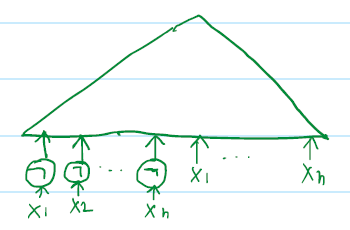
\includegraphics[scale=0.7]{images/image004.png}


\begin{corollary}[Repeated plucking]
With the parameters above, if we have $>M$ sets in a family, by repeated plucking we can reduce the number of sets to $\leq M$ (if we cannot apply plucking anymore we know by the Sunflower Lemma that the number of sets is $\leq M$).
\end{corollary}
We use the notation 
${\rm pluck}(Z)$ to denote the result of repeated plucking of a family $Z$ of sets, until $|Z| \leq M$.



% _____________________________________________________________________
\subsubsection{  Approximator Step Continued: Approximating OR and AND using Plucking}
% _____________________________________________________________________

We are finally ready to define precisely how to approximate OR and AND gates.
\begin{definition}[Approximators for $\lor$ and $\land$ gates]

\begin{description}
\item[The approximate for $g_1\lor g_2$:] Assume that $\gapx(g_1)=\APPX(\cX)$ and $\gapx(g_2)=\operatorname{\APPX}(\cY)$. Define 
$$\gapx(g_1\lor g_2):=\APPX(\operatorname{pluck}(\cX \cup \cY)).$$

\item[The approximate  for $g_1\land g_2$:]
Assume that $\gapx(g_1)=\APPX(\cX)$ and $\gapx(g_2)=\operatorname{\APPX}(\cY)$. Define 
$$\gapx(g_1\land g_2):=
    \APPX
        \left(
            \operatorname{pluck}
                \left\{
                    X_i \cup Y_j:
                        \left|
                            X_i \cup Y_j
                        \right| 
                        \leq l \text{ and } 
                        X_i \in \cX, Y_j \in \cY
                \right\}
       \right).
$$
\end{description}
\end{definition}


% NOT NEEDED:
% We show that: 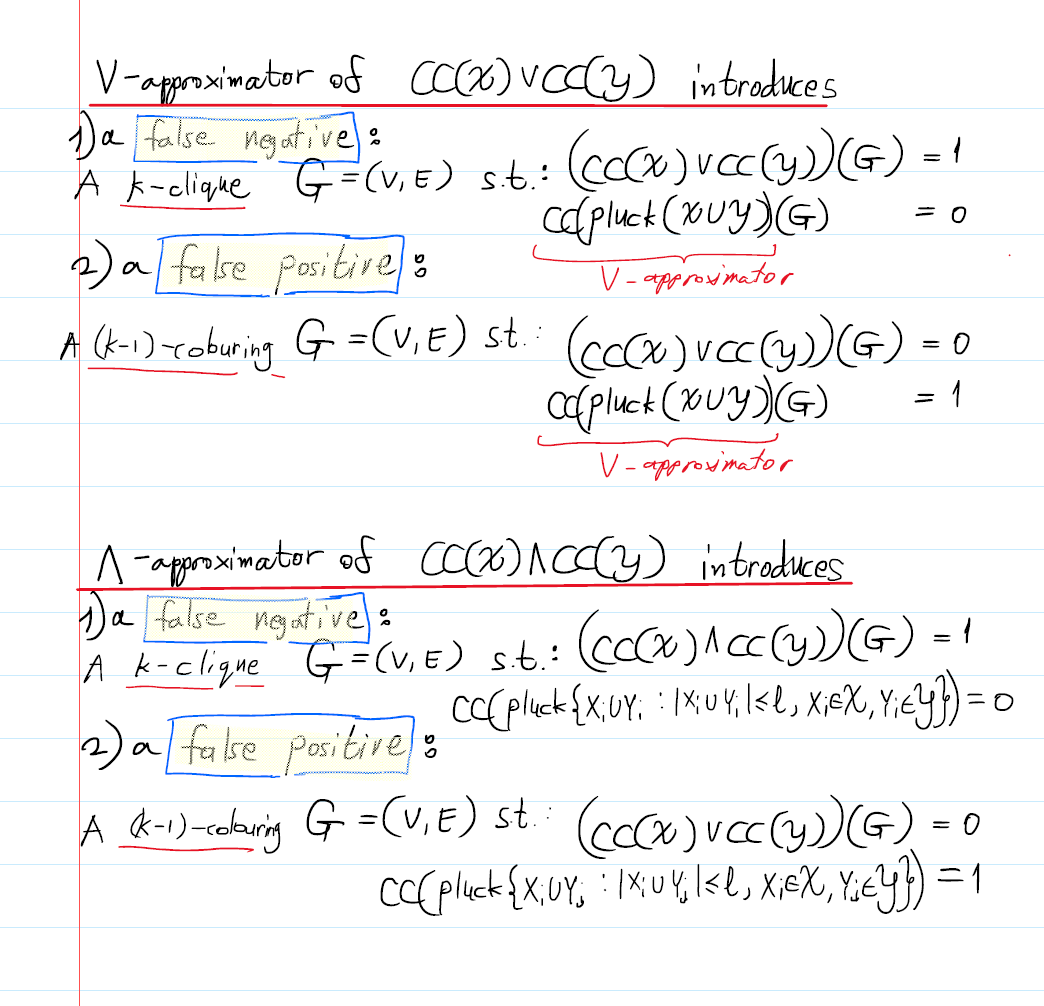
\includegraphics[scale=0.3]{image005.png}
% 
% $V$-approximator of $\operatorname{\APPX}(x) \vee \operatorname{\APPX}(y)$ introduces
% 1) a false negative:
% 
% A k-clique $G=(v, E)$ s.t.: $(\operatorname{cc}(x) \operatorname{vcc}(y))(G)=1$
% 2) a false positive:
% $\operatorname{cedpluck}(x \cup y)(G)=0$
% $V$-aterosimator
% $A(k-1)$-coburing $G=(v, E)$ s.t.
% 
% $$
% \begin{aligned}
% & (\operatorname{cc}(x) \vee \operatorname{cc}(y))(G)=0 \\
% & \frac{\operatorname{cc}(p l u c k(x \cup y))(G)}{V \text {-approvinator }}=1
% \end{aligned}
% $$
% 
% 
% 1 -apporimator of $\operatorname{\APPX}(x) \wedge \operatorname{\APPX}(y)$ introduces
% 1) a false negative:
% 
% A k-clique $G=(v, E)$ s.t: : $(\operatorname{cc}(x) \wedge \operatorname{cc}(y))(G)=1$
% 2) a false positive: $c c\left(P \mid\right.$ luck $\left.\left\{x_i\left|y_i:\left|x_i \cup y_i\right| \leq l, x_i \in X, y_i \in\right\}\right\}\right)=0$
% 
% $$
% \left.c c\left(p l u c k\left\{x_i \cup Y_j:\left|x_i \cup y_0\right| \leq l, x_i \in \chi, y_i \in\right\}\right\}\right)=1
% $$
%%%%% NOT NEEDED END

\para{Proof of \Cref{lem:new-false-positives}}


We need to show that each approximation step introduces at most $M^2 \frac{(k-1)^n}{2^p}$ false positives.


\case 1  OR-approximator.
We start with $\APPX\left(X_1, \ldots, X_m\right)$ and 
$\operatorname{\APPX}\left(Y_1, \ldots, Y_{m_m}\right)$ and consider a false positive introduced by

$$
\operatorname{\APPX}\left(\text{pluck}\left(X_1, \ldots, X_m, Y_1, \ldots, Y_{m^{\prime}}\right)\right) \text {. }
$$


That is, a $(k-1)$-colouring $G=(V, E)$ such that,
\begin{equation}\label{eq:991:24}
\operatorname{\APPX}\left(X_1, \ldots, X_m\right)(G)=0 
\quad \text{ and } ~~~\operatorname{\APPX}\left(Y_1, \ldots, Y_m\right)(G)=0
\end{equation}
while 
\begin{equation}\label{eq:960:30}
\operatorname{\APPX}\left(\operatorname{pluck}\left(X_1, \ldots, X_m, Y_1, \ldots, Y_{m^{\prime}}\right)\right)(G)=1 .
\end{equation}

We consider each plucking involved in \Cref{eq:960:30}, and bound from above the number of false positive introduced by this plucking. (Note that plucking is the only reason a false positive could be introduced.)


Consider a single plucking\footnote{It is fine to consider each single plucking, and count how many errors introduced in each such plucking. The reason is that once a plucking was done, we take the core $Z$ of some sunflower; and this new set $Z$ replaces all other set in the sunflower. Then we count the number of new errors introduced. Now, this $Z$ could  be replaced again in future pluckings, and we shall count the new errors introduced again.}: 
replace sunflower $\left\{Z_1, \ldots, Z_p\right\}$ by its core $Z$ (see \Cref{fig:pluck-stage}).

By \Cref{eq:991:24}: $Y_i$'s and $X_i$'s are all non-cliques in $G$.
Thus, by \Cref{eq:960:30}, $Z$ \emph{is} a new  clique
identified by the approximation and for every $i\in[p]$, the petal of $Z_i$ contains two nodes with the \emph{same colour} in $G$ (otherwise, there would have been a clique on some $Z_i$ in contrast to \Cref{eq:991:24}).

\begin{figure}[H]
    \centering
    \includegraphics[width=.6\linewidth]{images/clique3.png}
    \caption{Example}
    \label{fig:pluck-stage}
\end{figure}


We estimate the number of such $(k-1)$-colourings, using simple probability.
For this purpose we consider the following question:\ choosing a $(k-1)$-colouring of the nodes randomly and independently, \emph{what is the probability that every (petal of) $Z_i$ has repeated colours but the core $Z$ does not}?

As before, let $R(X)$ be the probability that $X$ has repeated colours.


$$
\operatorname{Pr}
\left[R\left(Z_1\right) \wedge 
\ldots \wedge R\left(Z_p\right) \wedge \neg R(Z)
\right] 
\leq \operatorname{Pr}\left[R\left(Z_1\right) \wedge \ldots \wedge R\left(Z_p\right) \mid \neg R(Z)\right]$$
(by definition of conditional probability $\operatorname{Pr}[A \land B]=\operatorname{Pr}[A \mid B] \cdot \operatorname{Pr}[B]$)

\begin{align*}
& =\prod_{i=1}^p \operatorname{Pr}\left[R\left(Z_i\right) \mid \neg R(Z)\right] 
\intertext{($Z_i$'s do not have common nodes, except those in $Z$, so given $\neg R(Z)$ the events $R(Z_i)$ are independent)}
& \leq \prod_{i=1}^p \operatorname{Pr}\left[R\left(Z_i\right)\right]\\
\intertext{(the probability of repetition of colours is increased if we do not restrict ourselves to colourings with no repetitions in the core $Z \subseteq Z_i$)}
& \leq \frac{1}{2^p}
\end{align*}
(because as we have seen before 
$\operatorname{Pr}[R(X)] \leq \frac{1}{2}$, for $|X|\le \ell$).


Finally, since the approximation step entails up to $\frac{2 M}{p-1}$ pluckings (each plucking decreases the number of sets by $\mathrm{p}-1$, and there are no more than $2M$ sets when we start), the lemma holds for the $\lor$ approximation step,  because (recall the total number of $(k-1)$-colouring is  $(k-1)^n$) 
$$
\frac{2 M}{p-1} \cdot \frac{(k-1)^n}{2^p} \leq
M^2 \cdot \frac{(k-1)^n}{2^p}  .
$$


\case 2 {$\land$-gate}.  Consider now an AND approximation step of approximators $\APPX(\cX)$ and $\APPX(\cY)$. It can be broken down in three phases, as follows. 

First, we form $\APPX(\{X \cup Y: X \in \cX, Y \in \cY\})$; this introduces no false positives, because any graph in which $X \cup Y$ is a clique must have a clique in both $X$ and $Y$, and thus it was accepted by both constituent approximators. 

The second phase omits from the approximator circuit several sets (those of cardinality larger than $\ell$), and can therefore introduce no false positives (because even less graphs are identified as having cliques). 

The third phase entails a sequence of fewer than $M^2$ plucking, during each of which, by the analysis of the OR case above, at most $2^{-p}(k-1)^{n}$ false positives are introduced. 

The proof of the lemma is complete: because at total we introduced $\leq M^2 \cdot \frac{(k-1)^n}{2^p}$ false positives.

\newpage



% Enable watermark from this point onward
\newpage\SetWatermarkText{DRAFT}


\para{Proof of Lemma \Cref{lem:new-false-negatives}}


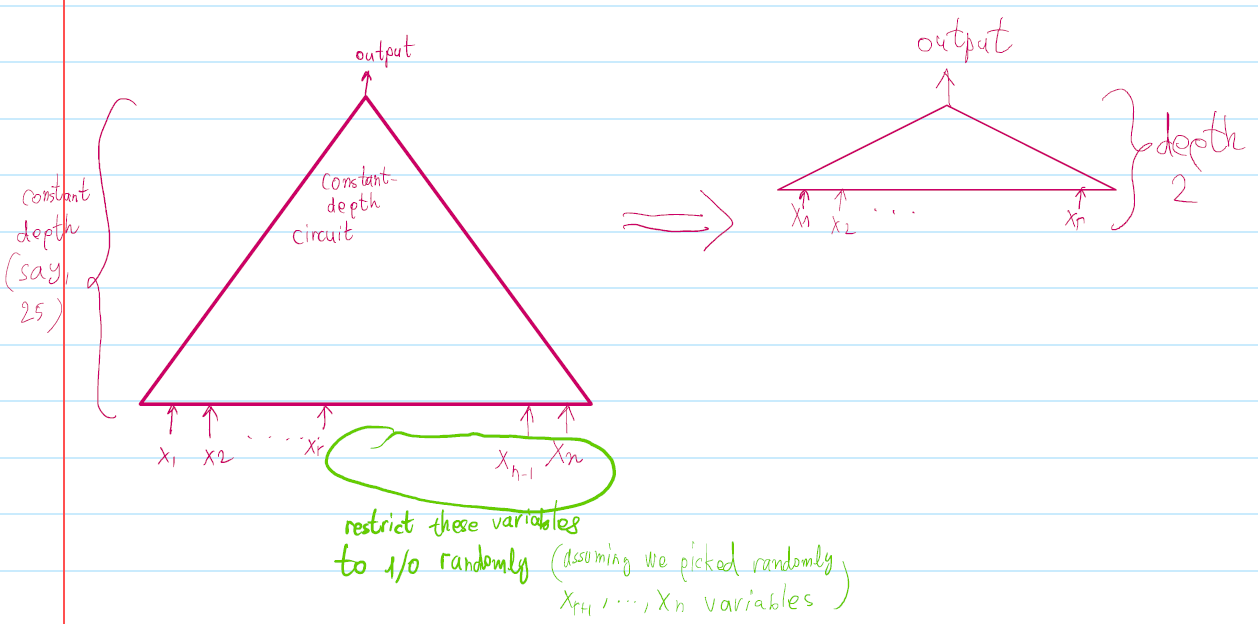
\includegraphics{images/image007.png}

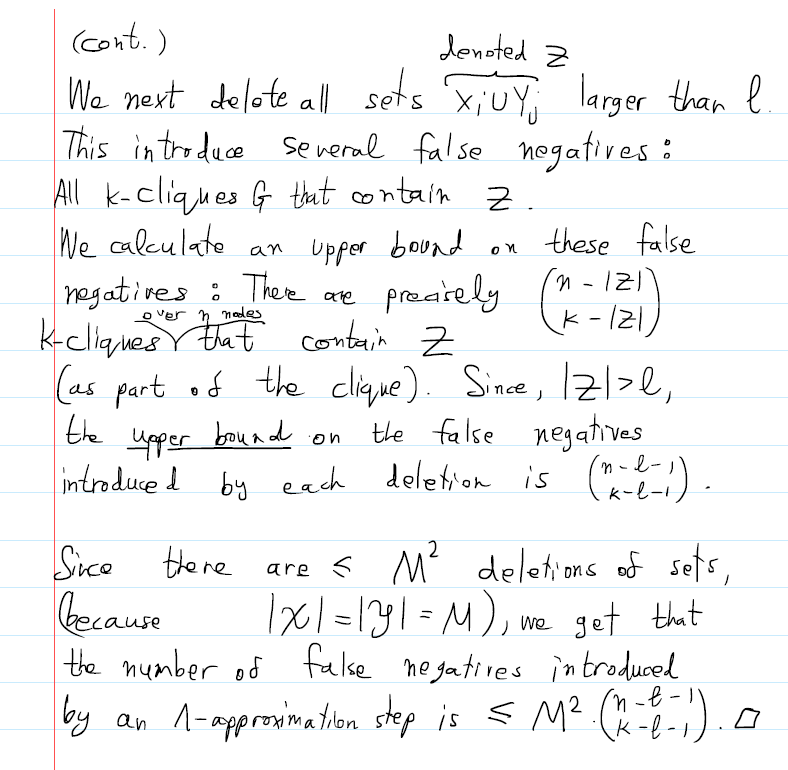
\includegraphics{images/image008.png}

\newpage

\iffalse
We need to show that each approximation step introduces $\leq M^2\binom{n-l-1}{k-l-1}$ false negatives.


Case $V_{:}$a false negative:
A $k$-clique $G=(v, E)$ st.: $(\operatorname{cc}(x) \vee \operatorname{ccc}(y))(G)=1$ (

$$
\underbrace{\operatorname{colpluck}(x \cup y)(G)}_{V \text {-aproximator }}=0
$$


This is impossible, because plucking only deletes sets and make them smaller; hence if (1) holds then (2) cannot.
Case 1:
A false negative:
A $k$-clique $G=(v, E)$ st: : $(\operatorname{cc}(x) \wedge \operatorname{cc}(y))(G)=1$

$$
\left.c\left(P / \mid u c k\left\{x_i \cup Y_j:\left|x_i \cup Y_i\right| \leq l, x_i \in \chi_{,}, Y_i \in\right\}\right\}\right)=0 \text { (2) }
$$


In the first stop we replace $c a(x) \wedge c(y)$ by $\APPX(\{X \cup Y: x \in X, y \in Y\})$.
Hence, if $G$ is a $K$-clique and both $X$ and $Y$ are each cliques in $G$, it must be that $X \cup Y$ is also a clique in $G(w h y$ ? ). Thus, no false negatives are introduced in this step.


$\frac{\text { (cont.) }}{\text { We next delete all sets } \overbrace{X_i \cup Y_j}^{\text {denoted }} Z}$ larger than $l$. This introduce several false negatives:
All $k$-cliques $G$ that contain $Z$.
We calculate an upper bound on these false negatives: There are precisely $\binom{n-|z|}{k-|z|}$ k-cliques er that contain $z$ (as part of the clique). Since, $|z|>l$, the upper bound on the false negatives introduced by each deletion is $\binom{n-l-1}{k-l-1}$.

Since there are $\leq M^2$ deletions of sets, (because $|\chi|=|y|=M$ ), we get that the number of false negatives introduced by $a_n 1$-approximation step is $\leq M^2 \cdot\binom{n-t-1}{k-l-1}$.
\fi

